\documentclass[a4paper,12pt]{article}

\usepackage{jheppub}
\usepackage{taro}

\title{Mathematical Methods in Physics}

\author[a]{Taro V. Brown}

\affiliation[a]{Department of Physics, UC Davis, One Shields Avenue, Davis, CA 95616, USA }


% e-mail addresses: one for each author, in the same order as the authors
\emailAdd{taro.brown@nbi.ku.dk}
\abstract{}
\begin{document} 
\maketitle
\flushbottom
\tableofcontents
\newpage
\section{Residue Calculus}
If $f(z)$ has a pole of order $m$ at $z=a$, thrn
\begin{equation}
\Res[f(z=a)]=\frac{1}{(m-1)!}\lim_{z\to a}\dv[m-1]{}{z}[(z-a)^mf(z)]
\end{equation}
Residue theorem:
If you have some domain with poles in them, you can pinch the conbtour of integration (since it doesn't affect the end results) around these poles. $f$ is analytic in the domain and on the boundary then
\begin{equation}
\oint _C \dd z  f(z)=2\pi i \sum_{a_i\in D}\Res[f(a_i)]\end{equation}
\underline{Jordan's Lemma:} Integrals along the real line, so the contour is just the real axis, so it is open:
\begin{equation}
	\sum_{-\infty}^{\infty}f(x)\dd x= \lim_{R\to \infty }\int_{-R}^{R}f(x)\dd x
\end{equation}
to convert this to a contour integral we have to close the open segment. This can be done by making a semi circle in either the upper or the lower half-plane.
\\
Jordan's Lemma says:
Let $C_R$ be a semicircle of radius R in e.g. upper half plane (UHP) and f is analytic in UHP and decays faster than $|z|^{-1}$ for $\arg(z)\in [0,\pi]$\footnote{This argument just specifies the UHP}, then
\begin{equation}
	\int_{C_R} \dd z e^{i\alpha z}\to 0 \text{ as } R\to \infty, \text{ for } \alpha > 0
\end{equation}
This gets an exponential damping through $i\alpha z=i\alpha \Re (z)-\alpha \Im(z)$, so the integral is bounded by $1/R$ which goes to zero when we take $R\to \infty$\\
\underline{Example:}
Rational functions
\begin{equation}
\int_{-\infty}^{\infty}\frac{p(x)}{q(x)}
\end{equation}
with $p$ and $q$ begin polynomials with $q$ being one degree higher than $p$, also assume $q$ doesn't have a zero along the real line. We can the write using J's Lemma
\begin{equation}
	\int_{-\infty}^{\infty}\frac{p(x)}{q(x)}=\lim_{R\to \infty}\int_{-R}^{R}\frac{p(x)}{q(x)}\to \oint_\gamma \dd z\frac{p(z)}{q(z)}=2\pi i \sum_{a_i\in\text{UHP}}\Res[\frac{p(a_i)}{q(a_i)}]
\end{equation}
where $\gamma$ is closed contour in either UHP or LHP with LHP giving a negative sign.\\
\underline{Example I}
\begin{equation}
\begin{aligned}
\int_{0}^{\infty}\frac{x^2}{(x^2+1)(x^2+9)}&=\frac{1}{2}\int_{-\infty}^{\infty}\frac{x^2}{(x^2+1)(x^2+9)}\\
&\to \frac{1}{2}\oint_\gamma \dd z \frac{z^2}{(z^2+1)(z^2+9)}
\end{aligned}
\end{equation}
This has zeros at $z^2=1$ and $z^2=9$ so 4 simple poles at $z=\{-3i,-i,i,3i\}$. We then include the residues at these poles, so
\begin{equation}
\begin{aligned}
	&\int_{0}^{\infty}\frac{x^2}{(x^2+1)(x^2+9)}\\
	&=\frac{1}{2}2\pi i \left\{
	\Res[\frac{z^2}{(z-i)(z+i)(z+3i)(z-3i)}]_{z=i}+	\Res[\frac{z^2}{(z-i)(z+i)(z+3i)(z-3i)}]_{z=3i}
	\right\}\\
	&=\frac{1}{2}2\pi i \left\{[\frac{z^2}{(z+i)(z+3i)(z-3i)}]_{z=i}+	[\frac{z^2}{(z-i)(z+i)(z+3i)}]_{z=3i}
	\right\}\\
	&=\frac{1}{2}2\pi i \left\{\frac{i^2}{(2i)(4i)(2i)}+\frac{(3i)^2}{(3i-i)(3i+i)(3i+3i)}]
	\right\}
\end{aligned}
\end{equation}
For simple pole one can just drop the pole part and evaluate the remainder at the pole to get the residue.\\
\underline{Example II}
Sin for imaginary values is just Sinh, so $\sin(a z)\to 0$ as $Im(z)\to \pm\infty$ depending on sign of $a:\pm$. Using $\sin(az)=\Im(e^{iz})$
\begin{equation}
	\begin{aligned}
		\int_{0}^{\infty}\frac{x \sin(a x)}{(x^4+4)}&=\Im \oint_\gamma \frac{z e^{iaz}}{(x^4+4)}
	\end{aligned}
\end{equation}
This has poles at $z=\pm 1 \pm i$ so
\begin{equation}
	\begin{aligned}
		\int_{0}^{\infty}\frac{x \sin(a x)}{(x^4+4)}&=\Im \oint_\gamma \frac{z e^{iaz}}{(x^4+4)}
	\end{aligned}
\end{equation}
...\\
...\\
\underline{Example III}
Functions of trig functions
\begin{equation}
	\begin{aligned}
		\int_{0}^{2\pi} \dd \theta F(\sin \theta, \cos \theta )
	\end{aligned}
\end{equation}
with $\sin\theta = \frac{z-\frac{1}{z}}{2}$ $\cos\theta = \frac{z+\frac{1}{z}}{2}$ and $\dd \theta=\frac{\dd z}{iz}$, so
\begin{equation}
	\begin{aligned}
		I=\oint_{|z|=1} \frac{\dd z}{iz} F(\frac{z-\frac{1}{z}}{2}, \frac{z+\frac{1}{z}}{2} )
	\end{aligned}
\end{equation}
E.g.
\begin{equation}
	\begin{aligned}
		\int_{0}^{2\pi} \dd \theta \frac{1}{1+a\cos \theta}\\
		&=\frac{2}{i}\oint_{|z|=1} \frac{\dd z}{iz\left[1+a\frac{z^2+1}{2z}\right]}\\
		&=\oint_{|z|=1} \frac{\dd z}{az^2+2z+a}\\
		&=\frac{2\pi}{\sqrt{1-a^2}}
	\end{aligned}
\end{equation}
the poles are at $z=-\frac{-1\pm\sqrt{1-a^2}}{a}$\\
\underline{Principal Value Prescription (Feynman $i\epsilon$ prescription)}
If one tries to integrate a function that blows up on the real line, e.g.
\begin{equation}
\int_{-\infty}^{\infty}\frac{f(x)}{x-a}, ~~~ a\in \mathds{R}
\end{equation}
The way to integrate this is by jumping the pole on axis either below or above, so the integral is slit into
\begin{equation}
	\int_{-\infty}^{a-\epsilon}\frac{f(x)}{x-a}+\int_{a+\epsilon}^{\infty}\frac{f(x)}{x-a}+\int_\Gamma\frac{f(x)}{x-a}
\end{equation}
with $\Gamma$ the contour around the pole on the axis. Then when closing the contour using Jordan's lemma, we have to close it in the plane opposite of the the one we jumped the pole in.
The integral then gives
\begin{equation}
I = P\mp i \pi f(a)
\end{equation}
where P is the principal part (the part of the integral that ignores the divergent pole at $a$). In Feynmans language:
\begin{equation}
\frac{1}{x-a\pm i\epsilon}=P(\frac{1}{x-a})\mp i \pi\delta(x-a)
\end{equation}
\underline{Example I}\\\\
Using the Feynman Prescription
\begin{equation}
\begin{aligned}
 \int_{0}^{\infty} \dd x\frac{\sin x}{x} &=\frac{1}{2}\Im\left[ \int_{-\infty}^{\infty} \dd x\frac{e^{ix}}{x}\right]\\
 &=\frac{1}{2}\Im\left[ \int_{-\infty}^{\infty} \dd x\frac{e^{ix}}{x-i\epsilon}\right]\\
  &=\frac{1}{2}\Im\left[P \int_{-\infty}^{\infty} \dd x\frac{e^{ix}}{x-i\epsilon}+i\pi \int_{-\infty}^{\infty} \dd x e^{ix}\delta(x)\right]\\
  &=\pi/2
\end{aligned}
\end{equation}
\underline{Example II}
\begin{equation}
	\begin{aligned}
		\int_{0}^{\infty} \dd k\frac{e^{ikx}}{k^2-m^2} &=\frac{1}{2}\Im\left[ \int_{-\infty}^{\infty} \dd x\frac{e^{ix}}{x}\right]
		&=-\frac{\pi}{x}\sin(m|x|)
	\end{aligned}
\end{equation}
Often the principal is real and since we take the imaginary part, the only contribution comes from the pole 
\section{Conformal Mapping}
Very useful tool in fluid dynamics, since it is very closely tied to solving the Laplace equation in two dimensions.\\
We have seen that if $f$ is analytic then $\Re(f)$ and $\Im (f)$ are harmonic, i.e. they satisfy Laplace's equations in $d=2$ automatically from Causchy-Riemann.
\\\\
\begin{equation}
z\to f(z)
\end{equation}
we can think of this map from some domain in z-plane to $w=f(z)$. It maps points to points. So if $f$ is analytic in the first region\footnote{We only consider simply connected domains, i.e. no holes in the domains.} then it is analytic after the map.
\\\\
\underline{Riemann Mapping Theorem}
The interior of any domain $\Omega$ (with more than 1 point on $\partial\Omega$), can be conformally mapped to the unit disc $D$ with the boundary being mapped to the unit circle. The map can be made unique by choosing to map a particular point $w_0\in \Omega$ to the origin of $D$ and by orienting a particular directions from $w_0$ to the real axis in $D$.
% TODO: \usepackage{graphicx} required
\begin{figure}[H]
	\centering
	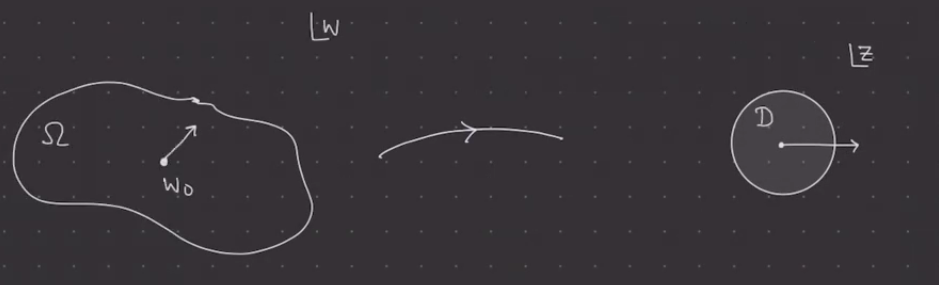
\includegraphics[width=0.7\linewidth]{3}
	\caption{}
	\label{fig:3}
\end{figure}
Let us imagine we are solving the following electrostatics problem:
\begin{equation}
\nabla^2\phi =-\delta(x)\delta(y)
\end{equation}
the potential in two dimensions behaves as
\begin{equation}
\phi\sim -\frac{1}{2\pi}\log r,~~~~~~r=\sqrt{x^2+y^2}
\end{equation}
We can map this to
\begin{equation}
	\Phi= -\frac{1}{2\pi}\log z
\end{equation}
The electrostatic potential with unit charge at $w_0$ and vanishing potential the boundary. From  $\phi$ in this domain we can construct $\Phi(w)$. Physically the situation is like punching a hole in a 2d conductor and placing a charge.
\begin{equation}
\Phi(w)=-\frac{1}{2\pi}\log (ze^{i\alpha})
\end{equation} 
is a conformal map from $w\to z$ plane which preserves the physical solution of the problem. Fixing $\alpha$, fixes a direction.\\\\
\begin{equation}
w=f(z)
\end{equation}
mapos the domain $\Omega$ to $D$. To get the inverse map $z=f^{-1}(w)$ we demand $f'(z)\neq 0$. IF
\begin{equation}
f=u+iv
\end{equation}
Then $\nabla^2u=\nabla^2 v=0$ and $u$ can be viewed as a solution to 3 dimensional Laplace equations if we have cylindrical symmetry. Let us use this to understand some problems we have already seen before.\\\\
Take $\phi=u= \Re f$ as the electrostatic potential, lines of constant $u$ gives equipotential. $v$ is field lines.\\\\
\underline{Example}
Uniform charge density wire along $z=x_3$. The equipotentials are circles and field lines go straight out.
\begin{figure}[H]
	\centering
	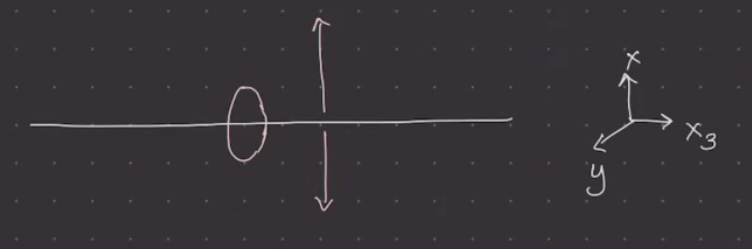
\includegraphics[width=0.7\linewidth]{4}
	\caption{}
	\label{fig:4}
\end{figure}
We have
\begin{equation}
\begin{aligned}
\Phi&=2\lambda \log z\\
\phi&=2\lambda \log r
\end{aligned}
\end{equation}
The equipotentials are $\Re[\Phi]=constant$ give circles in $x,y$ plane. Field lines come from $\Im(\phi)=2\lambda \Theta$.
\\\\
\underline{Example II}
\\\\
Two semi-infinite capacitor places at $y={\pi,-\pi}$ and hold them at constant potential $V(y=\pm \pi)=\pm \pi$. Sketching this, we now the equipotentials just go along the direction of the plates. We can use the exponential map to open it up to (almost) the whole complex plane, so taking $z\to1+z+e^z$. This maps a strip and maps it to the complex plane with two cuts. We can then solve the Laplace equation in the complex plane, i.e. we just get a linear function and the B.C.'s force the solutions to be non-zero.\\\\
The exponential map takes the complex plane and wraps it into a cylinder.
\begin{figure}[H]
	\centering
	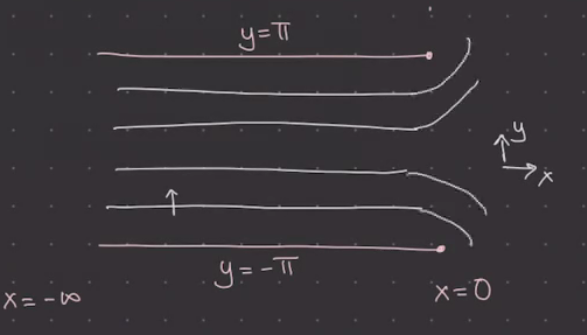
\includegraphics[width=0.7\linewidth]{5}
	\caption{}
	\label{fig:4}
\end{figure}
\begin{itemize}
\item Conformal maps are angle preserving (generally true in arbitrary dimensions)
\item In higher dimensions the full set of conformal maps is the group $SO(d,2)$ which is an extension of the Lorentz group (rotations and boost) SO($d-1,1$).
\item In 2 dimensions the conformal group is much richer: space of analytic maps. So any function $f(z)$ is a conformal transformation. This will be used later to construct interesting domain maps.
\item Subset of conformal maps: fractional linear transformations:
\begin{itemize}
	\item \begin{equation}
		w=\frac{az+b}{cz+d},~~~~~~ad-bc\neq0
	\end{equation}
	\item Translations $w=z+b$ (i.e. $c=0,d=1$)
	\item Scalings $w=\lambda z$ with $\lambda\in \mathds{R}_+$
	\item Rotations $w=e^{i\phi}z$
	\item Inversions $w=\frac{1}{z}$, analytic on $\mathds{C}/\{0\}$ maps interior of punctured disc to its exterior
 \end{itemize}
\end{itemize}
Think of $a,b,c,d$ parameterizing invertable $2\times 2$ matrices living in $GL(2,\mathds{C})$
\begin{equation}
A\begin{pmatrix}
a & b \\c& d
\end{pmatrix}
\end{equation}
If $\det A=ad-bc=1$ them we restrict to $SL(2,\mathds{C})$. \\\\
\underline{Riemann sphere}
The tranformations with $\det A=1$ transform the unit sphere onto it self. $\mathds{P}^1=\mathds{C}\cup \infty$. $S^2\subset R^3$, $\{x_1,x_2,x_3\}$. The sphere can be seen as a sterographic projection from the complex plane onto $S^2$
\begin{equation}
x_1=\frac{z+\bar z}{|z|^2+1},~~~~x_2=\frac{1}{i}\frac{z-\bar z}{|z|^2+1},~~~~x_3=\frac{|z|^2-1}{|z|^2+1}
\end{equation}
\begin{equation}
z=\frac{x_1+ix_2}{1-x_3}
\end{equation}\\\\
\subsection{How to find conformal maps}
First let us take some examples of maps:
\underline{Example I}\\\\
\begin{equation}
w=\frac{z-1}{z+1},~~~~z=\frac{w+1}{1-w}
\end{equation}
This map takes the right half of the $z$-plane to the unit disc in $w$\\\\
\underline{Example II}\\\\
\begin{equation}
\zeta= e^{i\phi}\frac{w-a}{\bar a w-1},~~~~~~|a|<1,~~~\phi\in (-\pi,\pi]
\end{equation}
This leaves the unit disc invariant.\\\\
The general way to find a conformal map is
\begin{itemize}
\item $w=f(z)$ are $\zeta=g(w)$ analytic then $\zeta= g\circ f(z)$ is a conformal map from $z\to \zeta$ planes
\end{itemize}
\underline{Example}\\\\
We want to map a strip in the z-plane to the unit disc. We know that the exponential function maps it to the right half plane
\begin{figure}[H]
	\centering
	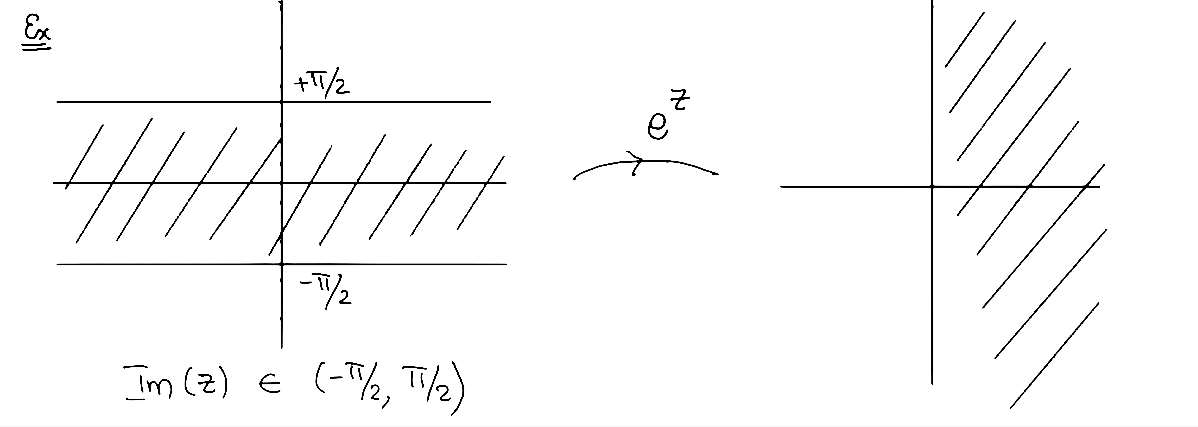
\includegraphics[width=0.7\linewidth]{7}
	\caption{}
	\label{fig:4}
\end{figure}
Now we can use the map from the half-plane to the unit sphere that we just saw and combine the two maps to get
\begin{equation}
\zeta = \frac{e^z-1}{e^z+1}
\end{equation}
\underline{Example}\\\\
To get the map from the UHP to the disc is just a combination of the right half plane map to unit disc, with a rotations:
\begin{equation}
\zeta=\frac{iz-1}{iz+1}
\end{equation}
\subsection{Applications in fluid dynamics}
We will focus on inviscid incompressible fluid and irrotational flows
\begin{equation}
\nabla\cdot \bm u=0,~~~~~~~~\nabla\times \bm u =0
\end{equation}
For 2d flow
\begin{equation}
\bm u=u_x(x,y)\hat e_x+u_y(x,y)\hat e_y
\end{equation}
The conditions on $\bm u$ imply that $u_x,u_y$ satisfy the CR relations. We can write the 2-dimensional vector field $u$ as a complex scalar $U$ as 
\begin{equation}
U(z)=u_x-iu_y
\end{equation}
Further we can write $\bm u=\nabla \phi$ and $\bm u=\nabla \times \begin{pmatrix}
1\\
1
\end{pmatrix}\chi$, with $\phi$ and $\chi$ being complex compliments and we can write
\begin{equation}
\Phi(z)=\phi(x,y)+i\chi(x,y)
\end{equation}
With
\begin{equation}
U(z)=\partial_z\Phi
\end{equation}
\underline{Example}\\\
\begin{figure}[H]
	\centering
	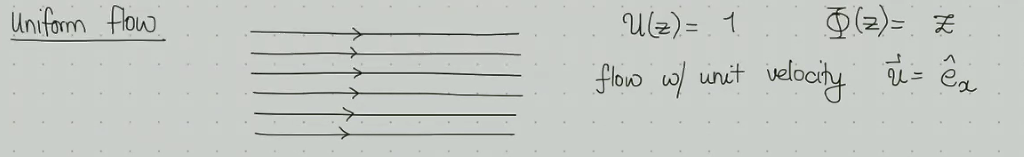
\includegraphics[width=0.8\linewidth]{8}
	\caption{}
	\label{fig:4}
\end{figure}
The streamlines are $y=c$ (constant lines) and the equipotentials are $x=c$. Now recall, analyticity of $\Phi(z)$ leads to $\grad \phi\cdot\grad \chi=0 $ since the velocity is the gradient of $\phi$ and it is tangent to $\chi=c$ then these are the level sets. If we were to add obstacles to the flow, these would be characterized by an absence of fluid flux into/out of the obstacle domain. 
\\\\
\underline{No flux condition}\\\\
$U$ is tangent to the boundary of the obstacle. $\phi$ should satisfy neumann bc at obstacle boundary
\begin{equation}
\pdv{\phi}{\bm n}
\end{equation} 
where $\bm n$ is the normal vector at the boundary.
\begin{figure}[H]
	\centering
	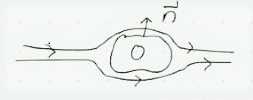
\includegraphics[width=0.6\linewidth]{9}
	\caption{}
	\label{fig:4}
\end{figure}
We will focus on flows which are asymptotically uniform, i.e. $\bm\to\hat e_x$ for $r\to \infty$ with some obstacle intermediate. Here are a few examples:
\begin{figure}[H]
	\centering
	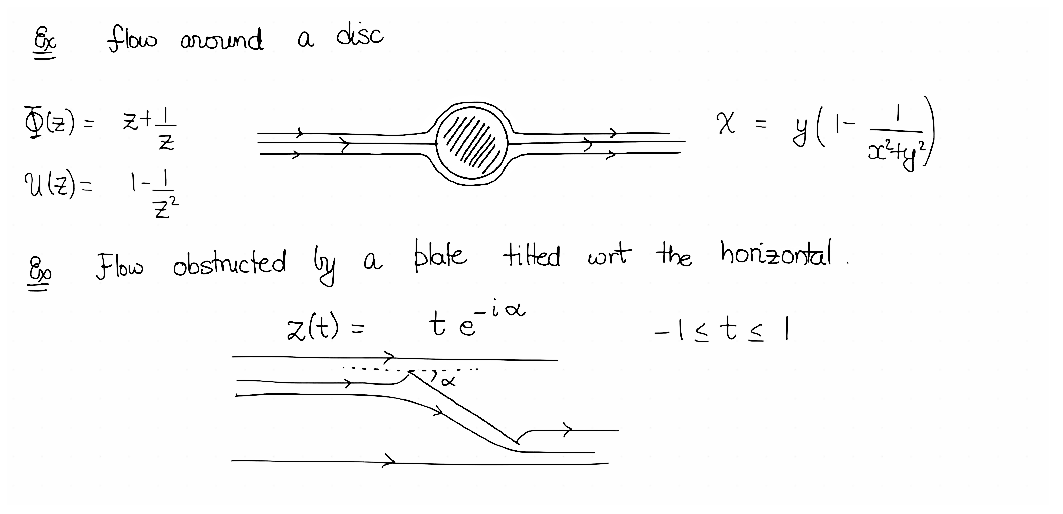
\includegraphics[width=0.9\linewidth]{10}
	\caption{}
	\label{fig:4}
\end{figure}
where $z(t)$ describes the locus of the plate
To solve the last example, we start by solving it for $\alpha=0$, so
\begin{equation}
z(t)=t,~~~~~~-1\leq t \leq 1
\end{equation}
here the solutions is clear since,
$\Phi(z)=z$. If $\alpha\neq 0$ we can solve it by rotating the plate using a conformal map. In aeronautics $\alpha$ is known as the attack angle. We will in this use the fact that rotations do not modify circular domains, which leads to the following trick:\\\\
The  Jakouwski map, mapped the unit disc to the real interval $[-1,1]$. Using this map we can go from the flow we know (at $\alpha=0$) to the unit disc, then rotate this using a rotational map, and finally map back to the $\alpha\neq 0$ solution.\\\\
The flow past a disc has then
\begin{equation}
\Phi(z)=\frac{1}{2}\left(z+z^{-1}\right)
\end{equation}
 We then rotate the disc by $\alpha$ using e.g. the map $w=e^{i\alpha}z$
 and so the jarkowski map goes to
 \begin{equation}
J(z)\to J(e^{-i\alpha})=\frac{1}{2}\left(e^{-i\alpha}w+\frac{e^{i\alpha}}{w}\right)
 \end{equation}
We then recollapse the disc by the inverse Joukoski map ($z(w)=w\pm\sqrt{w^2-1}$) and then finally rotate the solution back so that the streamlines are asymptotically horizontal, we lastly get:
\begin{equation}
\Phi(z)=e^{i\alpha}\left(z\cos \alpha -i\sin \alpha \sqrt{z^2-e^{-2i\alpha}}\right)
\end{equation}
As a pictorial example see below
\begin{figure}[H]
	\centering
	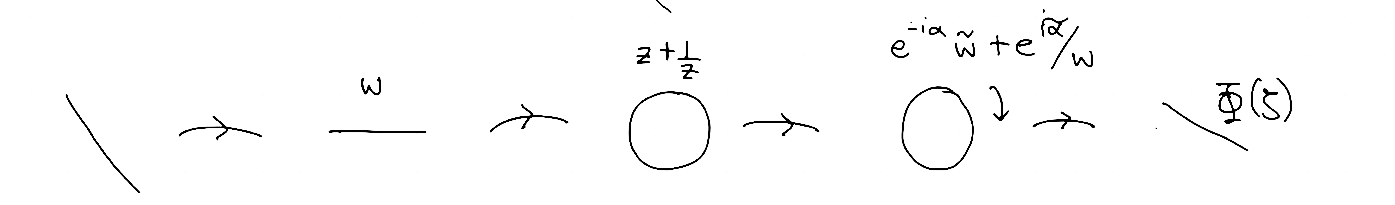
\includegraphics[width=0.9\linewidth]{11}
	\caption{}
	\label{fig:4}
\end{figure}
 %\underline{Example III}
%\\\\
%Two cylinders held at potentials $u$ and $v$ of equal size:
%\begin{figure}[H]
%	\centering
%	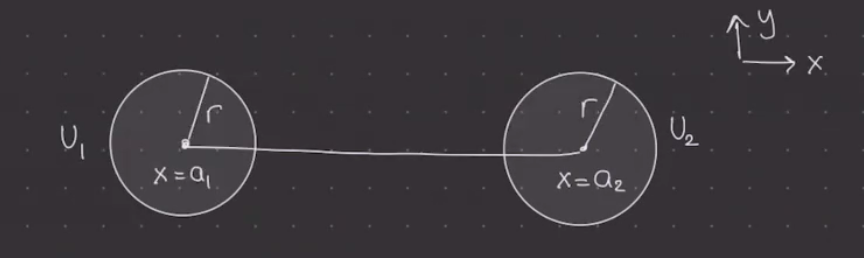
\includegraphics[width=0.7\linewidth]{6}
%	\caption{}
%	\label{fig:4}
%\end{figure}
%We want to find
\newpage
\section*{Homework 1\\\\
Taro V. Brown}\vspace*{1cm}
\section*{Problem 1}
\subsection*{Part a}
We compute
\begin{equation}
\oint_{|z|=3} \dd z\frac{4z-3}{z(z-2)}
\end{equation}
Inside the contour this has poles at $z=0$ and $z=2$ so using 
\begin{equation}
	\oint _C \dd z  f(z)=2\pi i \sum_{a_i\in D}\Res[f(a_i)]
\end{equation}
We get
\begin{equation}
\begin{aligned}
	\oint_{|z|=3} \dd z\frac{4z-3}{z(z-2)}=&2\pi i \left\{\Res[\frac{4z-3}{z(z-2)}]_{z=0}+\Res[\frac{4z-3}{z(z-2)}]_{z=2}\right\}\\
	=&2\pi i \left\{\frac{4\times 0-3}{(0-2)}+\frac{4\times 2-3}{2}\right\}\\
	=&2\pi i \left\{\frac{3}{2}+\frac{5}{2}\right\}\\	
	=&8\pi i 
\end{aligned}
\end{equation}
\subsection*{Part b}
Similarly
\begin{equation}
	\begin{aligned}
		\oint_{|z|=3} \dd z\frac{e^z}{(z-1)(z-2)}=&2\pi i \left\{\Res[\frac{e^z}{(z-1)(z-2)}]_{z=1}+\Res[\frac{e^z}{(z-1)(z-2)}]_{z=2}\right\}\\
		=&2\pi i \left\{-e+e^2\right\}\\
	\end{aligned}
\end{equation}
\section*{Problem 2}
\subsection*{Part a}
Computing
\begin{equation}
	\begin{aligned}
		\int_{0}^{\infty}\dd x\frac{2x^2-1}{x^6+1}
		=&	\frac{1}{2}\int_{-\infty}^{\infty}\dd x\frac{2x^2-1}{x^6+1}
		\\
		=&\frac{1}{2}\oint_{|z|=2} \dd z\frac{2z^2-1}{z^6+1}
	\end{aligned}
\end{equation}
$z^6+1$ has zero's within the contour at $z=\{i,(-1)^{\frac{1}{6}},(-1)^{\frac{5}{6}}\}$ and the residues can be computed by first factoring out the denominator 
\begin{equation}
(x^6+1)=(x-i)(x+i)\left(x-(-1)^{\frac{1}{6}}\right)\left(x+(-1)^{\frac{1}{6}}\right)\left(x-(-1)^{\frac{5}{6}}\right)\left(x+(-1)^{\frac{5}{6}}\right)
\end{equation}
and then applying the usual trick for first order poles. We get
\begin{equation}
\begin{aligned}
		\\
		=&\pi i
		 \left\{\Res[\frac{2z^2-1}{z^6+1}]_{z=i}+\Res[\frac{2z^2-1}{z^6+1}]_{z=(-1)^{\frac{1}{6}}}+\Res[\frac{2z^2-1}{z^6+1}]_{z=(-1)^{\frac{5}{6}}}\right\}\\
		=&\pi i \left\{\frac{i}{2}+\frac{1}{6}\left(-2i+(-1)^{\frac{1}{6}}\right)+\frac{1}{6}\left(-2i+(-1)^{\frac{5}{6}}\right)\right\}\\
		&=0
	\end{aligned}
\end{equation}

\subsection*{Part b}
For this integral we will be using $\sin n\theta =\frac{1}{2i}\left(z^n-z^{-n}\right)$, $\cos n\theta =\frac{1}{2}\left(z^n+z^{-n}\right)$ and $\dd \theta=\frac{1}{iz}\dd z$. We choose the contour $|z|=1$ since this includes all poles that show up. Computing we find
\begin{equation}
	\begin{aligned}
		\int_{0}^{\pi}\dd x\frac{\cos^2(3x)}{5-4\cos(2x)}
		=&\oint_{|z|=1}\frac{\dd z}{iz}\frac{\left(z^3+\frac{1}{z^3}\right)^2}{4 \left(1-2 \left(z^2+\frac{1}{z^2}\right)\right)}\\
		=&\oint_{|z|=1}\dd z \frac{i \left(z^6+1\right)^2}{8 z^9-4 z^7+8 z^5}\\
			=&2\pi i \left\{
			\Res[\frac{\left(z^6+1\right)^2}{8 z^9-4 z^7+8 z^5}]_{z=0}
			\right\}\\
			=&\frac{3\pi}{16}
	\end{aligned}
\end{equation}
\subsection*{Part c}
The following integral is a little tricky. First we rewrite the outer cosine at the real part of a complex function and combine the exponentials
\begin{equation}
\begin{aligned}
\int_{0}^{\pi}\dd x\, e^{\cos(x)}\cos[nx-i\sin(x)]&=\frac{1}{2}\Re\left[\int_{-\pi}^{\pi}\dd x\, e^{\cos(x)+inx-i\sin(x)}\right]\\
&=\frac{1}{2}\Re\left[\int_{-\pi}^{\pi}\dd x\, e^{inx}e^{e^{-ix}}\right]
\end{aligned}
\end{equation}
where we have used $e^{-ix}=\cos(x)-i\sin(x)$. Now
substituting $z=e^{-ix}$, which leads to $\dd z=-i e^{-ix} \dd x=-iz \dd x$
%%%%%%%%%%%%%%%%%%%%%%%%%%%%%%%%%%%%%%%%%%%%%%%%%%%%
\begin{equation}
	\begin{aligned}
\int_{0}^{\pi}\dd x\, e^{\cos(x)}\cos[nx-\sin(x)]&=\frac{1}{2}\Re\left[\int_{-\pi}^{\pi}\dd z\, \frac{e^{z}}{z^{(n+1)}}\right]\\
&=\frac{1}{2}\Re\left[\oint_{|z|=1}-i\dd z\, \frac{e^{z}}{z^{(n+1)}}\right]\\
	\end{aligned}
\end{equation}
This has an $n$'th order pole at $z=0$. We can find the residues using
\begin{equation}
	\Res[f(z=a)]=\frac{1}{(m-1)!}\lim_{z\to a}\dv[m-1]{}{z}[(z-a)^mf(z)]
\end{equation}
which in this case is particularly easy since we have an exponential function, so
\begin{equation}
	\begin{aligned}
		\int_{0}^{\pi}\dd x\, e^{\cos(x)}\cos[nx-\sin(x)]&=
		\Re\left [\pi \Res[\frac{e^{z}}{z^{(n+1)}}]_{z=0}\right]\\
		&=\frac{\pi}{n!}
	\end{aligned}
\end{equation}
\subsection*{Part d and Part e}
Lastly we have the two $\sinh$ integrals, with different contours. Let us first note that we have the Laurent series:
\begin{equation}
\frac{1}{\sinh z}=\frac{1}{z}-\frac{1}{6}z^2+\frac{7}{16}z^3+\cdots
\end{equation}
so that the combination
\begin{equation} \label{eq:sinh}
	\frac{1}{z^2\sinh z}=\frac{1}{z^3}-\frac{1}{6z}+\frac{7}{16}z+\cdots
\end{equation}
Further, we know that the zeroes of $\sinh z$ are at $n\pi i $, $n\in\mathds{Z}$ while for $z^2$ it is at $0$. This means that we for the contour $|z|=1$ only have to take the residue at $z=0$, while for $|z|=4$ also have to include the residue at $z=i\pi$. \eqref{eq:sinh} has a third order pole and a first order pole however since calculating the residue of the third order pole requires differentiating twice it's residue is just zero and we only need the contribution from the first order pole
\begin{equation}
\begin{aligned}
\oint_{|z|=1}\dd z\,\frac{1}{z^2\sinh z}  &=2\pi i \Res[\frac{1}{z^2\sinh z}]_{z=0}\\
&=2\pi i \left[-\frac{1}{6}\right]\\
&=-\frac{\pi i}{3}
\end{aligned}
\end{equation}
For the larger contour we, as mentioned, have to include the residue at $i\pi$ and $-i\pi$. The residue at this point be calculated using
\begin{equation}
\Res[\frac{p(z)}{q(z)}]_{z=a}=\lim_{z\to a}\left[\frac{p(z)}{q'(z)}\right]
\end{equation}
where $q(z)$ has a pole at $z=a$ and $p(z)$ does not. Hence taking $q(z)=\sinh(z)$ and $p(z)=z^2$  we have
\begin{equation}
\begin{aligned}
\Res[\frac{1}{z^2}\frac{1}{\sinh z}]_{z=i \pi}&=\lim_{z\to i\pi }\left[\frac{1}{z^2}\frac{1}{\cosh z}\right]\\
&=\frac{1}{\pi^2}
\end{aligned}
\end{equation}
and
\begin{equation}
	\begin{aligned}
		\Res[\frac{1}{z^2}\frac{1}{\sinh z}]_{z=-i \pi}&=\lim_{z\to -i\pi }\left[\frac{1}{z^2}\frac{1}{\cosh z}\right]\\
		&=\frac{1}{\pi^2}
	\end{aligned}
\end{equation}
So the total contour integral is
\begin{equation}
	\begin{aligned}
		\oint_{|z|=4}\dd z\,\frac{1}{z^2\sinh z}  &=2\pi i \left\{
		\Res[\frac{1}{z^2\sinh z}]_{z=0}+\Res[\frac{1}{z^2\sinh z}]_{z=i\pi}+\Res[\frac{1}{z^2\sinh z}]_{z=-i\pi}
		\right\}\\
		&=2\pi i \left[-\frac{1}{6}+\frac{1}{\pi^2}+\frac{1}{\pi^2}\right]\\
		&=2\pi i \left[-\frac{1}{6}+\frac{2}{\pi^2}\right]
	\end{aligned}
\end{equation}
\section*{Problem 3}
Using Cauchy's integral formula
\begin{equation}
	\begin{aligned}
f(a)&=\frac{1}{2\pi i}\oint_{z=|R|} \dd z\,\frac{f(z)}{z-a}
	\end{aligned}
\end{equation}
We can subtract the following term since it is zero inside this contour by Cauchy's theorem
\begin{equation}
	\begin{aligned}
		0&=\frac{1}{2\pi i}\oint_{z=|R|} \dd z\,\frac{f(z)\bar a}{ R^2-\bar az}
	\end{aligned}
\end{equation}
So we get
\begin{equation}
	\begin{aligned}
		f(a)&=\frac{1}{2\pi i}\oint_{z=|R|} \dd z\,\left[\frac{f(z)}{z-a}-\frac{f(z)\bar a}{ R^2-\bar az}\right]\\
		&=\frac{1}{2\pi i}\oint_{z=|R|} \dd z\,f(z)\frac{R^2-\bar a a}{(z-a)(R^2-\bar az)}\\
	\end{aligned}
\end{equation}
Where we have put everything on a common denominator in the last term. Expanding this denominator and writing $|a|^2=\bar a a$ we find
\begin{equation}
	\begin{aligned}
		f(a)
		&=\frac{1}{2\pi i}\oint_{z=|R|} \frac{\dd z}{z}\,f(z)\frac{R^2-|a|^2}{R^2-2\Re(a\bar z)+|a|^2}
	\end{aligned}
\end{equation}
Then letting $a=re^{i\theta}$ and integrating around the contour by setting $z=Re^{i\phi}$, $0\leq \phi \leq 2\pi$ \footnote{Note that we in the above have used $\bar z=z^{-1}$}. Further we have $\dd z=iRe^{i\phi}\dd \phi=iz\dd \phi$ and $|a|^2=r^2$, then
\begin{equation}
	\begin{aligned}
f(re^{i\theta})&=\frac{1}{2\pi i}\int_{0}^{2\pi} \dd \phi\,f(Re^{i\phi})\frac{R^2-r^2}{R^2-2Rr\cos(\theta-\phi)+r^2}
	\end{aligned}
\end{equation}
Since $f$ was assumed analytic inside the disc, this solves the Laplace equation in this region since it can be written in terms of harmonic functions through the Cauchy-Riemann conditions.
\section*{Problem 4}
\subsection*{Part a}
We have the Navier-Stokes equation:
\begin{equation}
\partial_t \bm u+\bm u\cdot  \nabla\bm u=-\nabla \left(\frac{1}{\rho} p- V\right)+\nu\nabla^2 \bm u
\end{equation}
Taking the curl on both sides we use the fact that the curl of a gradient of scalar is zero 
\begin{equation} \label{eq:ns}
	\partial_t \bm \omega+\nabla\times(\bm u \cdot \nabla\bm u)=+\nu\nabla^2 \bm w
\end{equation}
Furtherm, since $\nu=0$ in this case
\begin{equation} \label{eq:ns}
	\partial_t \bm \omega+\nabla\times(\bm u \cdot \nabla\bm u)=0
\end{equation}
Then using the fact that
\begin{equation}
\bm u \cdot \nabla\bm u=\frac{1}{2}\nabla u^2-\bm u\times (\nabla \times \bm u)=\frac{1}{2}\nabla u^2-\bm u\times \bm \omega
\end{equation}
we can rewrite
\begin{equation}
\begin{aligned}
\nabla\times(\bm u \cdot \nabla\bm u)&=\frac{1}{2}\nabla\times\nabla u^2-\nabla\times (\bm u\times \bm \omega)\\
&=\nabla\times (\bm \omega \times \bm u)\\
&=(\bm u \cdot \nabla)\bm\omega -(\bm \omega  \cdot \nabla)\bm u +\bm\omega (\nabla\cdot \bm u)+\bm u (\nabla\cdot \bm \omega )\\
&=(\bm u \cdot \nabla)\bm\omega -(\bm \omega  \cdot \nabla)\bm u
\end{aligned}
\end{equation}
where the we have used $\nabla\cdot \bm u=0$ and $\bm u(\nabla \cdot \bm \omega)=\bm u(\nabla \cdot (\nabla \times \bm u))=0$ in the third line. Inserting this back into \ref{eq:ns}:
\begin{equation} \label{eq:ns2}
	\partial_t \bm \omega+(\bm u \cdot \nabla)\bm\omega =(\bm \omega  \cdot \nabla)\bm u
\end{equation}
Or in index notation:
\begin{equation} \label{eq:ns2}
	\partial_t \omega_i+ u ^j \partial_j\omega_i = \omega^j  \partial_j u_i
\end{equation}
\subsection{Part b}
If $\bm \omega =\nabla\times \bm u =0$, we could write
\begin{equation}
\bm u=\nabla \phi
\end{equation}
Since the equation
\begin{equation}
\nabla\times \nabla\phi =0
\end{equation}
is automatically satisfied. This is similar to the gauge potential in electrodynamics. Further from the incompressibility we know $\phi$ satisfies the Laplace equation
\begin{equation}
\nabla\cdot u=\nabla^2 \phi=0
\end{equation}
\subsection*{Part c}
First we insert $u=\nabla\phi$ into Navier-Stokes equation. Note that the following terms can be rewritten as:
\begin{equation}
\begin{aligned}
\bm u \cdot \nabla\bm u&=\frac{1}{2}\nabla u^2-\bm u\times (\nabla \times \bm u)\\
&=\frac{1}{2}\nabla u^2-\bm u\times (\nabla \times \nabla\phi)\\
&=\frac{1}{2}\nabla u^2
\end{aligned}
\end{equation}
So that we after inserting get:
\begin{equation}
	\nabla \partial_t \phi+ \frac{1}{2}\nabla \phi^2+=-\nabla \left(\frac{1}{\rho} p+ V\right)
\end{equation}
Which we can write as
\begin{equation}
	\nabla \left(\partial_t \phi+\frac{1}{2} u^2+\frac{p}{\rho} + V\right)=0
\end{equation}
This means that we can write the part in parenthesis as a constant in space but function of time $F(t)$
\begin{equation}
 \left(\partial_t \phi+\frac{1}{2} u^2+\frac{p}{\rho} + V\right)=F(t)
\end{equation}
Finally since we can just absorb the time-dependence through a shift in $\phi(t)\to\phi'$ we can write this as
\begin{equation} \label{eq:flow}
\partial_t \phi'+\frac{1}{2} u^2+\frac{p}{\rho} + V=0
\end{equation}
\subsection*{Part d}
We have already shown that since we have irrotational flow, i.e. $\nabla\times \bm u=0$ we can write the flow field as a gradient
\begin{equation}
\begin{aligned}
	u_x&=\partial_x \phi\\
	u_y&=\partial_y \phi
\end{aligned}
\end{equation}
Further, since we have an incompressible fluid, i.e. $\nabla\cdot\bm  u=0$ we can write it as a "curl" of a scalar\footnote{Since there doesn't exist such thing as a curl of scalar function, the use of curl in this case should be taken as meaning \begin{equation}
\bm u=\nabla\times \begin{pmatrix}
1\\1
\end{pmatrix}\chi
\end{equation}}
\begin{equation}
\begin{aligned}
u_x&=\partial_y \chi\\
u_y&=-\partial_x \chi
\end{aligned}
\end{equation}
since it automatically satisfies $\nabla\cdot u=0$. We see that in this case we can use either $\phi$ or $\chi$ to solve \eqref{eq:flow} and that further
\begin{equation}
	\begin{aligned}
		\partial_x \phi&=\partial_y \chi\\
		\partial_y \phi&=-\partial_x \chi
	\end{aligned}
\end{equation}
These are just the Cauchy-Riemann relations and so we we can construct an analytic function out of these, known as the stream function
\begin{equation}
\Phi=\phi+i\chi
\end{equation}
This stream-function also solves \eqref{eq:flow} since the derivatives act linearly on it as a consequence of the Cauchy-Riemann relations. This can be seen by multiplying the two sides
\begin{equation}
-\partial_x\phi\partial_x\chi=\partial_y\phi\partial_y\chi
\end{equation}
implying $(\nabla\phi)\cdot (\nabla\chi)=0$. This also implies that $\phi$ is tangent to the level sets of $\chi$. As mentioned, the terms with derivatives on $\Phi$ then become linear combinations of $\phi$ and $\chi$ and so $\Phi$ must solve the equation as well:
\begin{equation}
|\nabla \Phi|^2=(\nabla \phi+i\nabla\chi)(\nabla \phi-i\nabla\chi)=(\nabla\phi)^2+(\nabla\chi)^2
\end{equation}
\subsection*{Part e}
Here we refer to the Milne-Thomson theorem which can be used to obtain the stream-function in the case of a cylindrical obstacle through
\begin{equation}
\tilde \Phi=\Phi(z)+\bar \Phi\left(\frac{a^2}{z}\right)
\end{equation}
In this case we will assume a uniform flow with speed $u=\frac{1}{2}$ in the $x$-direction and so we have the stream-line function $\Phi(z)=\frac{1}{2}z$ and place the cylinder with $a=1$, so we get 
\begin{equation}
	\begin{aligned}
	\tilde \Phi&= \frac{1}{2}\left(z+\frac{1}{z}\right)
	\end{aligned}
\end{equation}
On the curve $|z|=1$, we have $\bar z = \frac{1}{z}$ and so the imaginary part of $\Phi$ is zero. Since $\chi=constant$ represented the constant flow streamlines, the surface of the cylinder has become a streamline and the flow doesn't penetrate this surface. This also means that the solutions holds for $|z|>1$ as prescribed in the problem.
%%%%%%%%%%%%%%%%%%%%%%%%%%%%%%%%%%%%%%%%%%%%%%%%%%
\newpage
\section*{Homework 2\\\\
	Taro V. Brown}\vspace*{1cm}
\section*{Problem 1}
\section*{Problem 2}
The transformation that takes the unit disc to the unit disc is the linear fractional tranformation
\begin{equation}
\zeta= e^{i\phi}\frac{z-\alpha}{\alpha z-1},~~~~~~|\alpha|<1,~~~~~-\pi<\phi < \pi
\end{equation}
The rotation part $e^{i\phi}$ obviously just maps points on the disc to other points on the disc, while the linear fraction part moves the origin from $z=0$ to $\zeta=a$. We can show that this maps to the unit disc if $|\zeta|<1$ so that every point in the domain lies within the disc. First we note that
\begin{equation}
|z-a|^2=(z-a)(\bar z-\bar a)
\end{equation}
\end{document}
